%
% Documento: Abordagem e modelagem do Problema
%

\chapter{Abordagem e Modelagem do Problema: Malhas de Controle}
\label{chap:abordagememdelo}
%Existem diversas maneiras de se implementar um sistema como este, tanto do ponto de vista do sistema distribuído e sua rede de comunicação, quanto do ponto de vista de controle e realimentação das malhas. Neste capítulo faz-se um detalhamento da abordagem do problema, do funcionamento do sistema como um todo e a modelagem escolhida para abordar os problemas. 

%Para resolução deste problema, primeiramente, estudou-se as possibilidades da implementação do mesmo em uma rede descentralizada, onde não tem-se um mestre definido, apenas uma sociedade de robôs que conforme precisam executar uma tarefa, vão recrutando e formando uma frota. No entanto, concluiu-se que, apesar de viável, a implementação de um sistema distribuído descentralizado seria muito complexo para ser abordado no período deste trabalho, que tem como objetivo principal o estudo de estratégias de controle de formação de múltiplos robôs móveis. Para tanto, foi adotada uma estrutura de rede centralizada denominada 'Mestre/Escravo' e um controle em cascata, utilizado para modularizar o problema e assim, tornar mais simples a implementação e o entendimento do mesmo. 

%Como citado no \autoref{chap:Metod}, serão utilizadas duas abordagens diferentes, uma para resolver apenas o primeiro problema e a outra uma abordagem mais genérica que permite adaptação para resolução de ambos os problemas. A primeira abordagem, utilizará uma malha de controle de velocidade e uma malha de controle que será responsável pela comunicação entre os robôs e definirá a velocidade de cada robô, baseado na posição dos outros integrantes da frota.

%Já a segunda abordagem
Como já dito no \autoref{chap:Metod}, foi escolhida uma estratégia que atende à resolução de ambos os problemas\ a qual, consiste em três malhas de controle: a primeira e mais interna será responsável pelo controle da velocidade angular de cada roda, para se chegar à posição (\emph{x,y}) desejada; a segunda, malha intermediária, será responsável para que cada robô chegue à um determinado ponto (\emph{x,y}) no espaço, portanto, será responsável por corrigir o posicionamento do robô (A primeira e a segunda malhas serão implementadas em cada um dos robôs da frota); a terceira malha e, portanto, a mais externa, é responsável pela coordenação da frota, fornecendo a cada robô as informações necessárias para que o mesmo saiba o ponto (\emph{x,y}) que deve rastrear para consolidar e manter a formação.

Faz-se então neste capítulo um detalhamento das malhas de controle utilizadas e das modificações realizadas para que a estratégia atenda a ambos os problemas, bem como uma descrição de como funcionam as malhas responsáveis pela comunicação e pelo controle de formação para a resolução de cada um dos problemas. Faz-se também um levantamento dos possíveis problemas que podem surgir na implementação do sistema.   
%Faz-se então neste capítulo, primeiramente, a modelagem do problema, para que então, possa-se simular e implementar o problema. Para estabelecer o modelo matemático do problema, será considerado o modelo de robô mostrado na \autoref{fig:robo}.

\section{Malha de Controle 1: Velocidade Angular das Rodas}
\label{sec:malha1 } 
Como já dito anteriormente, este sistema de controle consiste em um controle de três malhas, e agora será abordada a primeira malha. Ela controla os motores para atingir a velocidade angular desejada de cada roda ($\omega_{dr},\omega_{dl}$). Ou seja, a malha de controle vai receber a velocidade linear e angular que se deseja imprimir no robô e retornar a "potência" que deve ser aplicada a cada um dos motores para se atingir as velocidades desejadas, como pode ser observado na \autoref{fig:malha1}.

\begin{figure}[!htb]
	\centering
	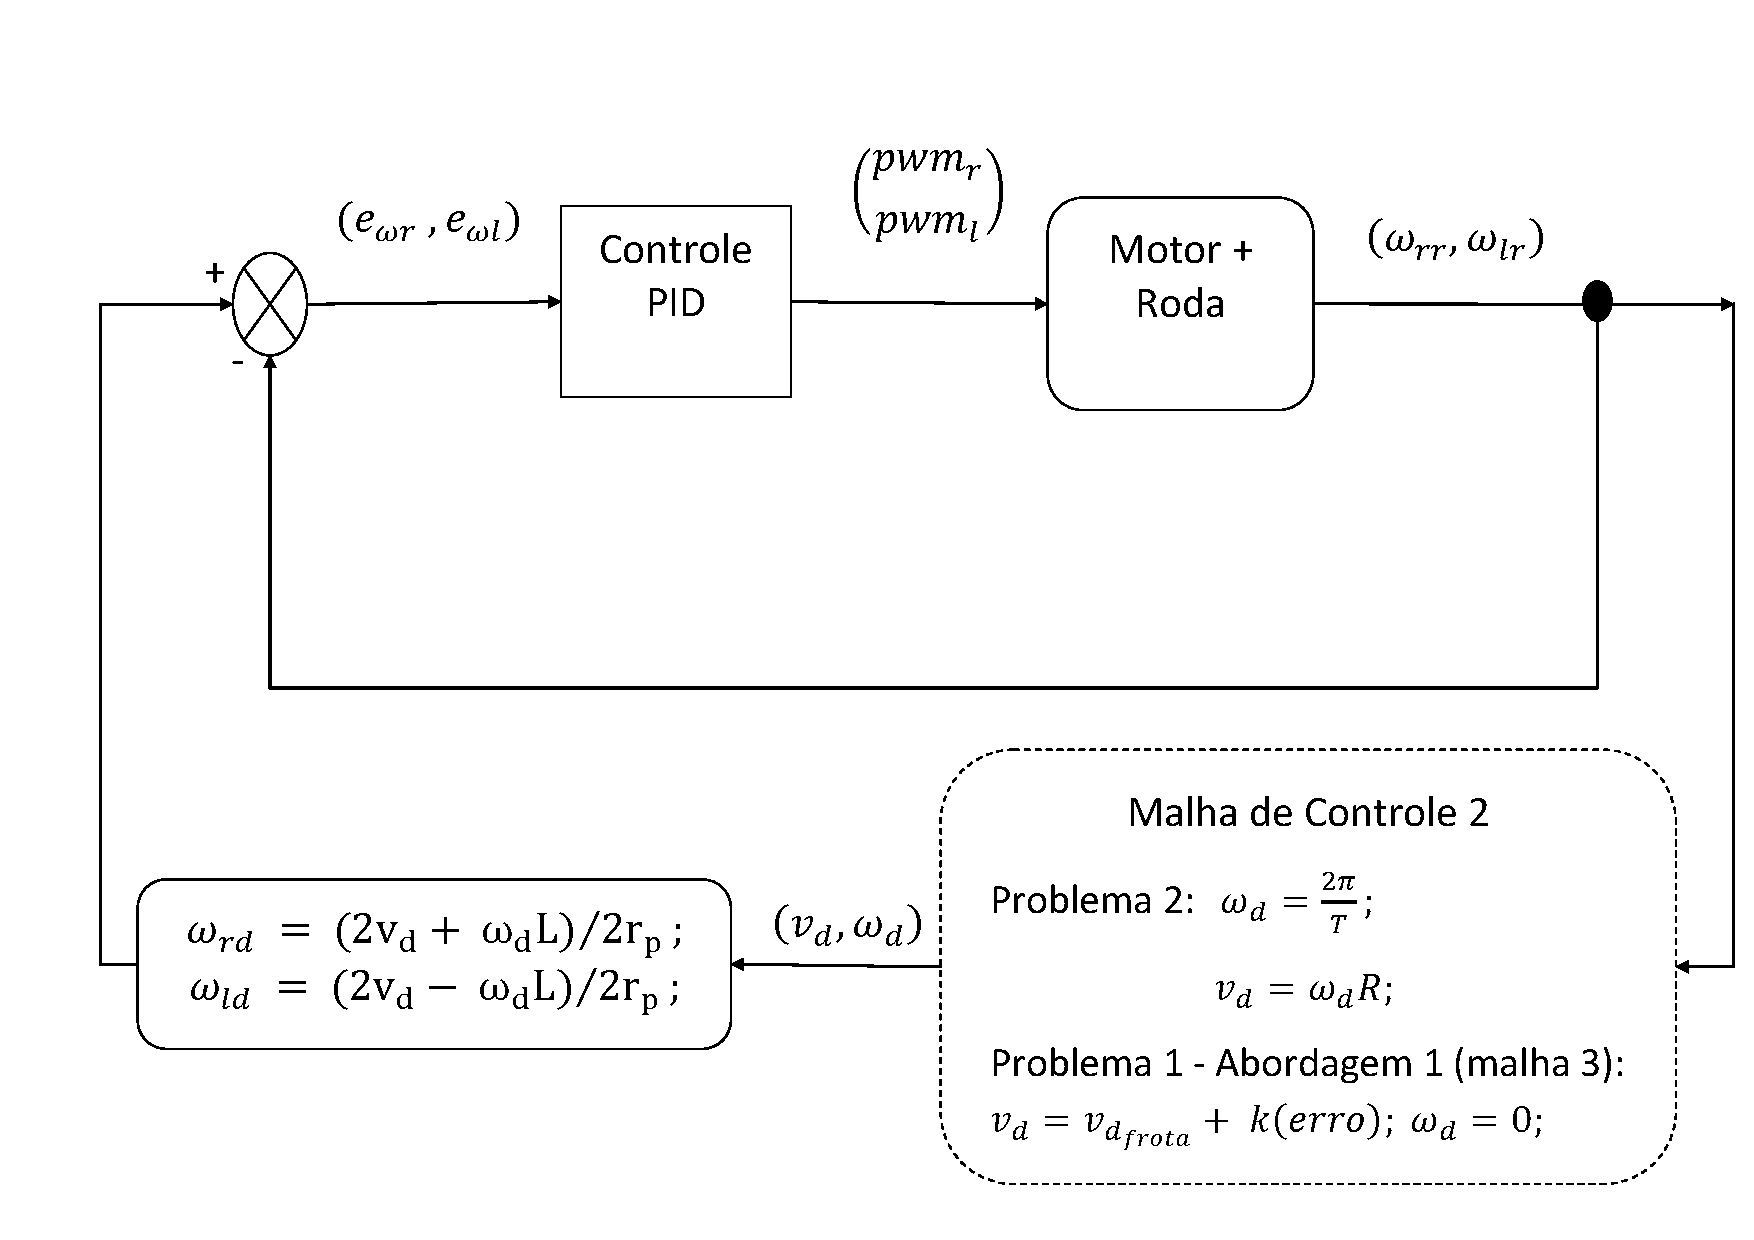
\includegraphics[width=1.0\textwidth]{./04-figuras/malha1}
	\caption{Primeira malha de Controle do Sistema - Controle da velocidade angular}
	\label{fig:malha1}
\end{figure}

É importante ressaltar que como o robô não é um elemento pontual\footnote{Veja a \autoref{fig:sistEst} para visualizá-lo como um elemento não pontual, que depende da variação de velocidade de cada roda para definir a velocidade e o sentido do robô.}, como considerado na \autoref{sec:modMatematico} ao descrever as equações do modelo, temos que descrever a velocidade angular (\emph{$\omega$}) e linear (\emph{$v$}) do robô em função de cada roda, para sabermos a potência a ser aplicada em cada uma delas para que o robô obtenha a velocidade e o sentido desejados.

A partir daí o %módulo 
microcomputador embarcado calcula a velocidade angular desejada de cada roda, como indicado nas equações abaixo que, por sua vez, são oriundas das equações (\ref{eq:vConv}) e (\ref{eq:wConv}):
\begin{subequations}
\begin{equation}
\omega_{dr} = \dfrac{2v + \omega_{d}L}{2r_{p}}	
\label{eq:velocangulardireita}
\end{equation} 
\begin{equation}
\omega_{dl} = \dfrac{2v - \omega_{d}L}{2r_{p}}	
\label{eq:velocangularesquerda}
\end{equation} 
\label{eq:convVelAngRodas}
\end{subequations}
onde:
\begin{itemize}
	\item $v_d$ é a velocidade linear desejada do robô ($m/s$);
	\item $\omega_{dr}$ é a velocidade angular desejada da roda direita ($rad/s$);
	\item $\omega_{dl}$ é a velocidade angular desejada da roda esquerda ($rad/s$);
	\item $r_{p}$ o raio da roda ($m$);
	\item $L$ o tamanho do eixo das rodas do robô ($m$).	
\end{itemize}

Com a velocidade angular de cada roda  do robô, estimada a partir dos dados fornecidos pelos \emph{encoders}, é calculado o erro das velocidades dado por:%, como mostrado nas equações abaixo, 
\begin{equation}
e_{wr} = \omega_{dr} - \omega_{rr}
\label{eq:errVelAngDireita}
\end{equation} 
\begin{equation}
e_{wl} = \omega_{dl} - \omega_{rl}
\label{eq:errVelAngEsquerda}
\end{equation} 
onde:
\begin{itemize}
	\item $e_{wr}$ e $e_{wl}$ são os erros da velocidade angular da roda direita e esquerda, respectivamente;
	\item $\omega_{rr}$ e $\omega_{rl}$ é a velocidade angular real da roda direita e esquerda, respectivamente.
\end{itemize}
E o controlador os retorna as ações de controle que serão passadas como potência para cada uma das rodas.	

\section{Malha de Controle 2: Posicionamento}
\label{sec:malha2} 
Para que a malha de controle 3, que consiste no controle de formação do sistema multiagente funcione, primeiramente é necessário implementar o controle de posicionamento de cada robô. Ou seja, para que o robô cumpra a missão, é necessário que a malha de controle de formação passe para cada robô os parâmetros necessários para o ajuste da estrutura, tais como, posicionamento, velocidade e número de robôs da frota. Cada robô por sua vez, deve conseguir se posicionar corretamente de acordo com a posição recebida pela malha de controle 3, o que só será possível se a malha de controle 1 conseguir controlar adequadamente os motores para que eles imprimam a velocidade correta em cada roda.

Como pode ser visto na \autoref{fig:esq2}, o problema a ser resolvido pela segunda malha de controle consiste em, dado um sistema de coordenadas cartesianas, onde têm-se um robô móvel de posição (\emph{$x_{r},y_{r}$}), cuja orientação (\emph{$\theta$}) é indicada em relação ao eixo \emph{x} do sistema, %onde pretende-se 
fazer com que o robô chegue ao ponto desejado (\emph{$x_{d},y_{d}$}), recebido da malha de controle 3. Para tanto, a malha 2 funciona da seguinte maneira: Recebe da malha 3 os parâmetros necessários para o cálculo da posição desejada do robô (\emph{$x_{d},y_{d}$}), e a partir daí é determinado o erro de posição do robô (\emph{$e_{x},e_{y}$}), fazendo-se a diferença entre a posição desejada e a posição real do robô (\emph{$x_{r},y_{r}$}), que é obtida através dos \emph{encoders} do LEGO\textregistered, que se mostrou suficientemente precisos.

\begin{equation}
e_{r} = r_{d} - r_{r}
\label{eq:errr}
\end{equation}
\begin{equation}
e_{x} = x_{d} - x_{r}
\label{eq:errx}
\end{equation}
\begin{equation}
e_{y} = y_{d} - y_{r}
\label{eq:erry}
\end{equation}

Através do erro de posicionamento do robô, encontra-se o ângulo de orientação desejado\footnote{Para fins de implementação é altamente recomendável o uso da função \emph{atan2} que mapeia o ângulo de orientação para o intervalo entre $-\pi$ e $\pi$, contemplando todos os quatro quadrantes do plano $xy$. Essa função é utilizada neste trabalho para calcular o ângulo de orientação desejado e limitar o erro do ângulo de orientação.}, dado por: %(\emph{$\theta_{d}$}), como mostrado na \autoref{eq:thetad}. 
\begin{equation}
\theta_{d} = \arctan\left(\dfrac{e_{y}}{e_{x}}\right)
\label{eq:thetad}
\end{equation}
Então, o erro do ângulo de orientação do robô é obtido, através da %\autoref{eq:errtheta} abaixo.
equação indicada abaixo: 
\begin{equation}
e_{\theta} = \theta_{d} - \theta_{r}
\label{eq:errtheta}
\end{equation}

O erro do ângulo de orientação (\emph{$e_{\theta}$}) é passado para o controlador que retorna a velocidade linear e angular da ação de controle, que será passada para a malha mais interna (malha 1). %Posteriormente, será feita uma comparação entre os controladores \emph{PI} e \emph{PID} e será definido o controlador a ser utilizado nesta malha.

\begin{figure}[!htb]
	\centering
	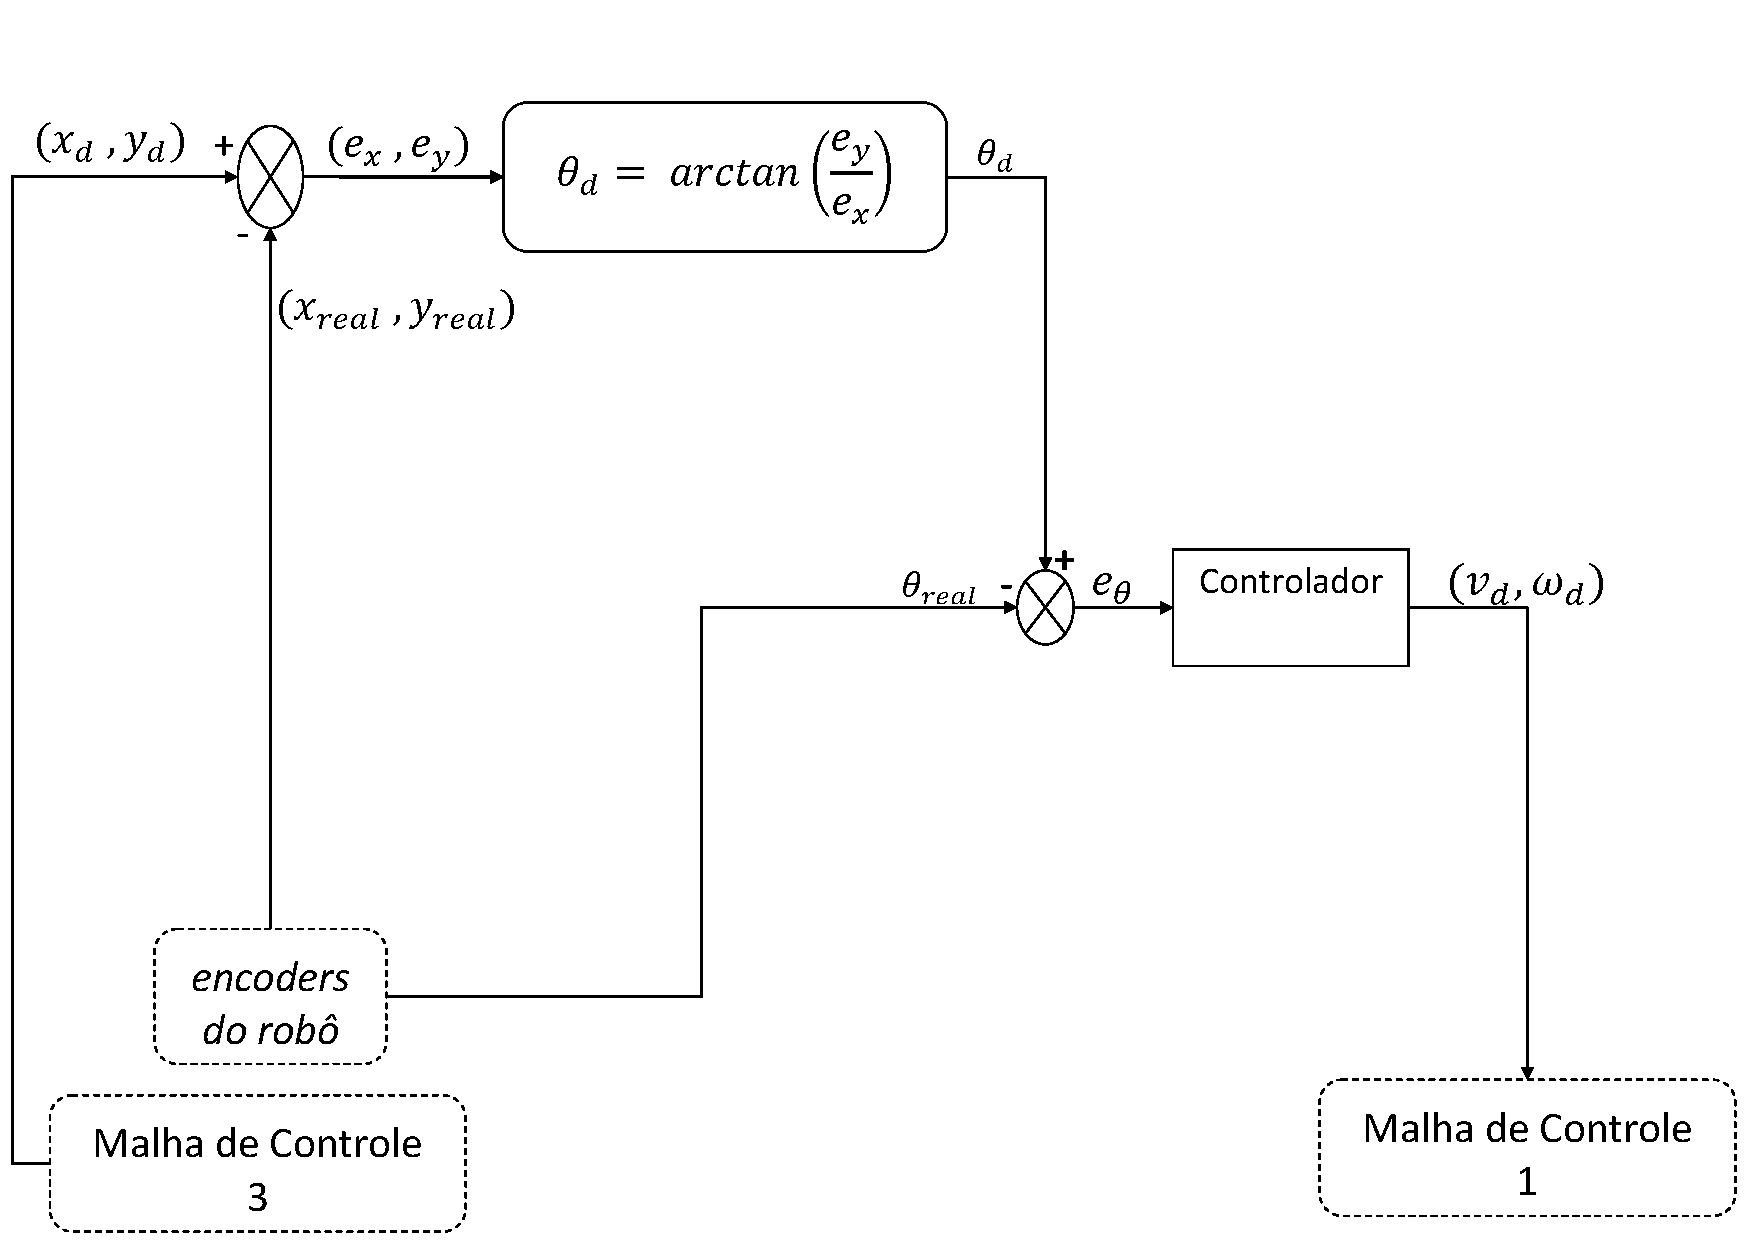
\includegraphics[width=1.0\textwidth]{./04-figuras/malha2}
	\caption{Segunda malha de Controle do Sistema - Controle de Posicionamento}
	\label{fig:malha2}
\end{figure}

\section{Malha de Controle 3: Controle de formação}
\label{sec:malha3 }
A malha de controle de formação tem como função estabelecer a comunicação entre os robôs, enviando os dados necessários para que se estabeleça a formação da frota. Além disso, ela utiliza as informações recebidas para estabelecer a posição em que o robô deve assumir naquele instante. Existem duas formas de se fazer esse controle, uma delas consiste em centralizar este controle de formação no mestre e enviar para o restante da frota apenas a posição desejada já calculada; já a outra consiste na troca de informações entre os agentes do sistema sem sobrecarregar o mestre.

No caso do primeiro problema (varredura de área em paralelo), é necessário que cada robô saiba a posição no eixo das abscissas de todos os outros robôs e a partir daí calcule a posição desejada, ou seja, um determinado robô recebe a posição dos outros robôs da frota e utiliza a \autoref{eq:xdp1} para obter a posição desejada do robô naquele instante, que é passada para a malha de controle intermediária, que por sua vez calcula o erro de posicionamento e envia para a malha de controle de velocidade interna as velocidades que devem ser assumidas pelo robô para que o mesmo possa alcançar a posição desejada e cumprir os objetivos estabelecidos. É importante ressaltar que, a depender da rede implementada, como é o caso deste trabalho em que a rede é centralizada e os robôs escravos não se comunicam entre si, essas informações devem ser passadas de um robô para o outro sempre através do mestre. %entre a frota através do mestre.

Já no caso do segundo problema (circulação de um robô), as informações que cada robô deve possuir para assumir a formação da frota são: número de robôs da frota, numeração que aquele robô representa na frota e posição do alvo. A partir daí é possível utilizar as \autoref{eq:posDesejada_p2} para se obter a posição desejada para que aquele robô contribua positivamente para a formação da estrutura da frota. Como pode ser visto na \autoref{eq:posDesejada_p2}, a definição da posição desejada leva em consideração o tempo, o que é um problema na aplicação prática, visto que não há uma sincronia entre os relógios dos robôs. Dessa forma, para contornar este problema, será levado em consideração o relógio do mestre, sendo necessário que essa variável também seja repassada ao restante da frota. 

%É importante notar que esta malha de controle não é uma malha fechada, ou seja, ela não possui realimentação. Esta malha apenas controla as informações e para quais robôs as mesmas devem ser enviadas, além de calcular a posição desejada utilizando-se das equações já mostradas anteriormente. 







%Ou seja, deseja-se circular o alvo em um período de \emph{T} segundos, a malha de controle de velocidade vai receber a velocidade angular desejada ($ \omega _{d} $), que é uma derivação do período de circulação desejado, como mostrado na equação abaixo:



 

